\section{Pipeline}

\begin{figure}[t]
  \begin{center}
  \subfigure[Serialized Laundry Loads]{
\includegraphics[width=\textwidth]{images/laundryserial}} 
  \subfigure[Pipelined Laundry Loads]{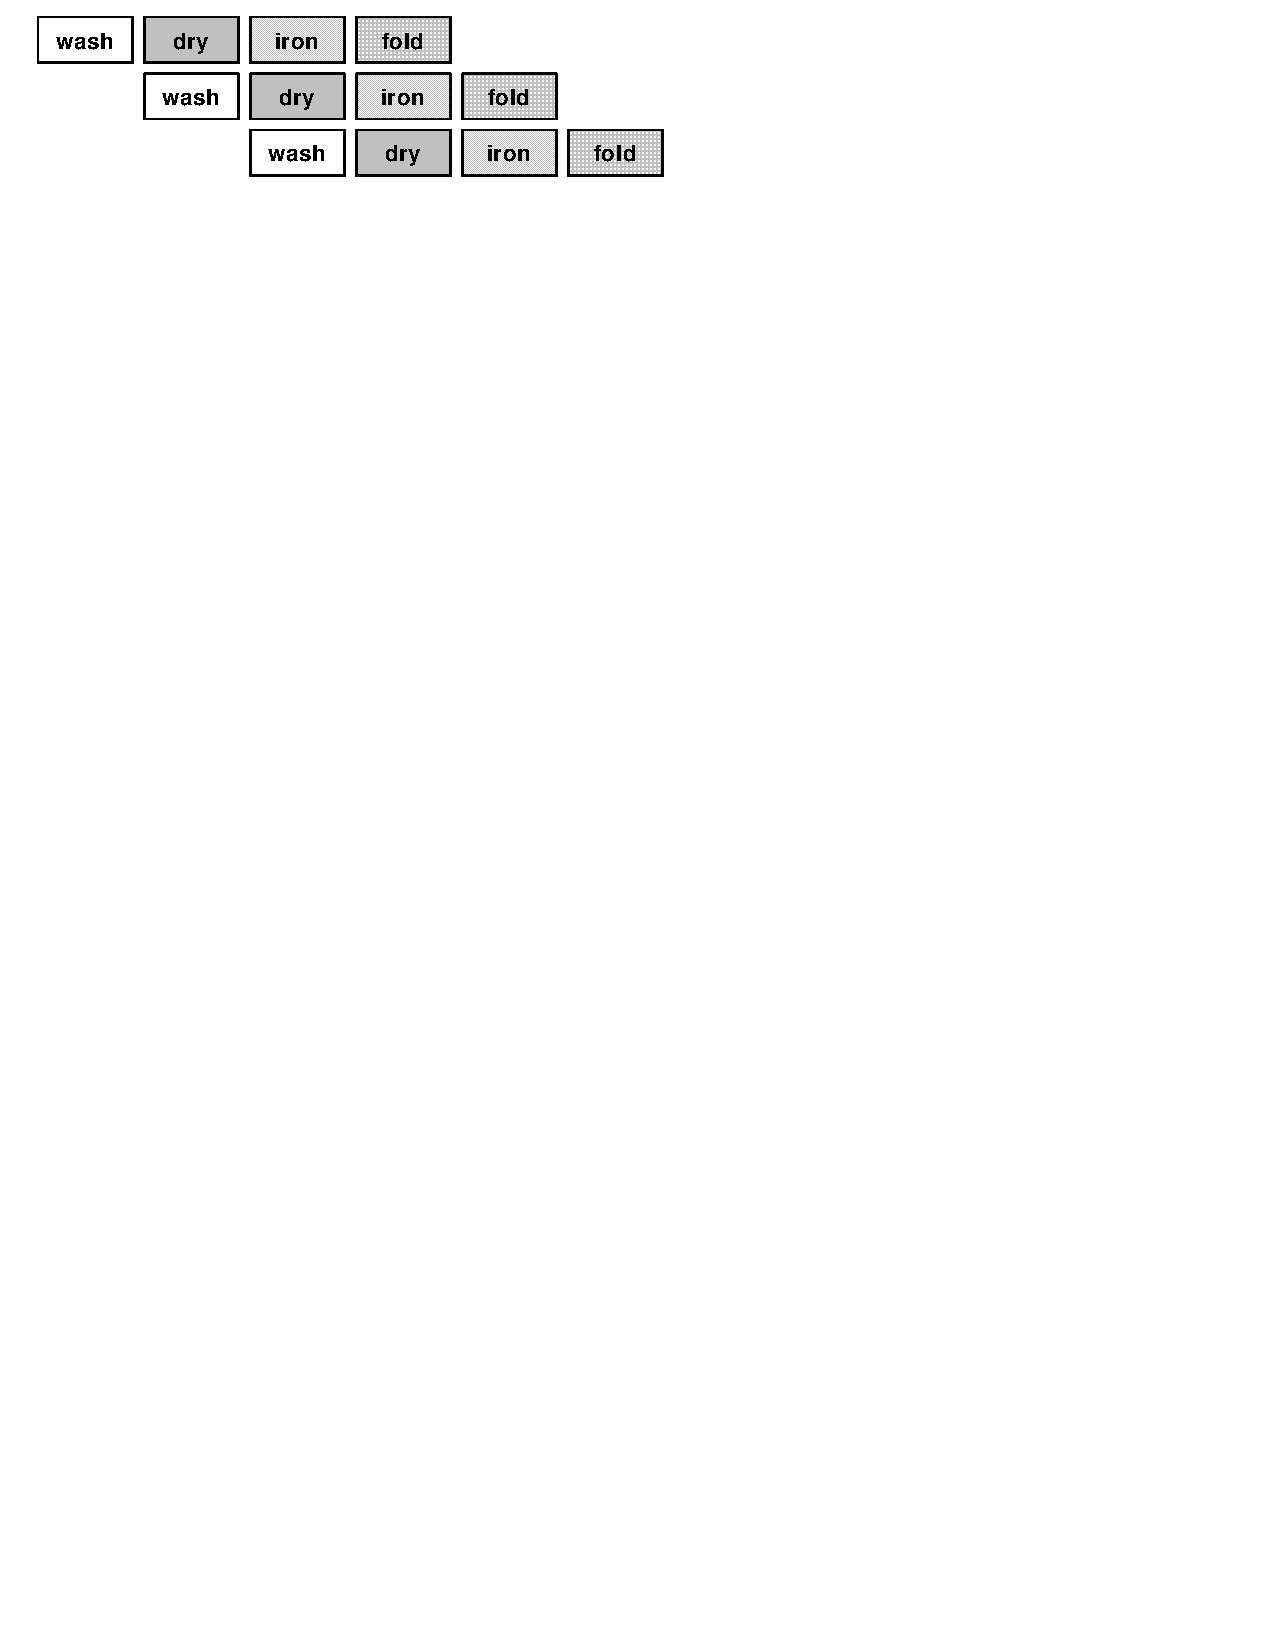
\includegraphics{images/laundrypipe}} 
  \caption{Pipeline in Laundry}
  \label{fig:laundry}
  \end{center}
\end{figure}

The pipeline design pattern adds concurrency to applications by splitting up a
previously single threaded task into multiple tasks \cite{Vermeulen95}. This is
done by treating sub-phases of a task as independent tasks themselves. If this
is done, then each sub-phase still believes it is operating in a single thread,
but it is happening concurrently with all of the other sub-phases.

Consider the classic laundry pipeline example shown in Figure \ref{fig:laundry}.
Let's say your task is to complete three loads of laundry from start to finish.
You can do each of these loads serially, or you can pipeline the process. For
this example, let's split the task into four phases: wash, dry, iron, and fold. 
With this pipeline in place, we can add concurrency to the laundry task. We
start by washing load one. When that finishes, we dry the first load and start 
load two in the wash. When that finishes, we iron load one, dry, load two, and
start the wash on load three. This process continues for the three loads with 
added concurrency in each step. As you can see, doing laundry this way is much
faster because the added concurrency allows you to finish the entire job as a
whole much faster.

In Coursebook, we can exploit the pipeline design pattern to improve the
perceived response time. This is made possible with a new web application
strategy called AJAX, or \textbf{A}synchronous \textbf{J}avascript \textbf{A}nd
\textbf{X}ML.

With Javascript and new functionality introduced by the AJAX design paradigm,
it is now possible to build richer web applications with more functional and
interactive UI's \cite{Crane05}. By writing Javascript code in an AJAX fashion,
a software developer can transform a web browser into a pull flow, active reader
for pipeline processing \cite{Vermeulen95}.

\subsection{Pipeline in Coursebook}

To improve the perceived response time of our Coursebook web application, we can
introduce pipelining into the loading of our UI. Instead of downloading the
entire page and rendering it all at once, we split this task into four 
sub-phases and pipeline them. For Coursebook, we define these phases for the
pipeline:

\singlespacing
\begin{enumerate}
  \item download bits
  \item update the DOM (Document Object Model)
  \item parse the HTML
  \item render the page
\end{enumerate}
\doublespacing

\begin{figure}[t]
  \begin{center}
  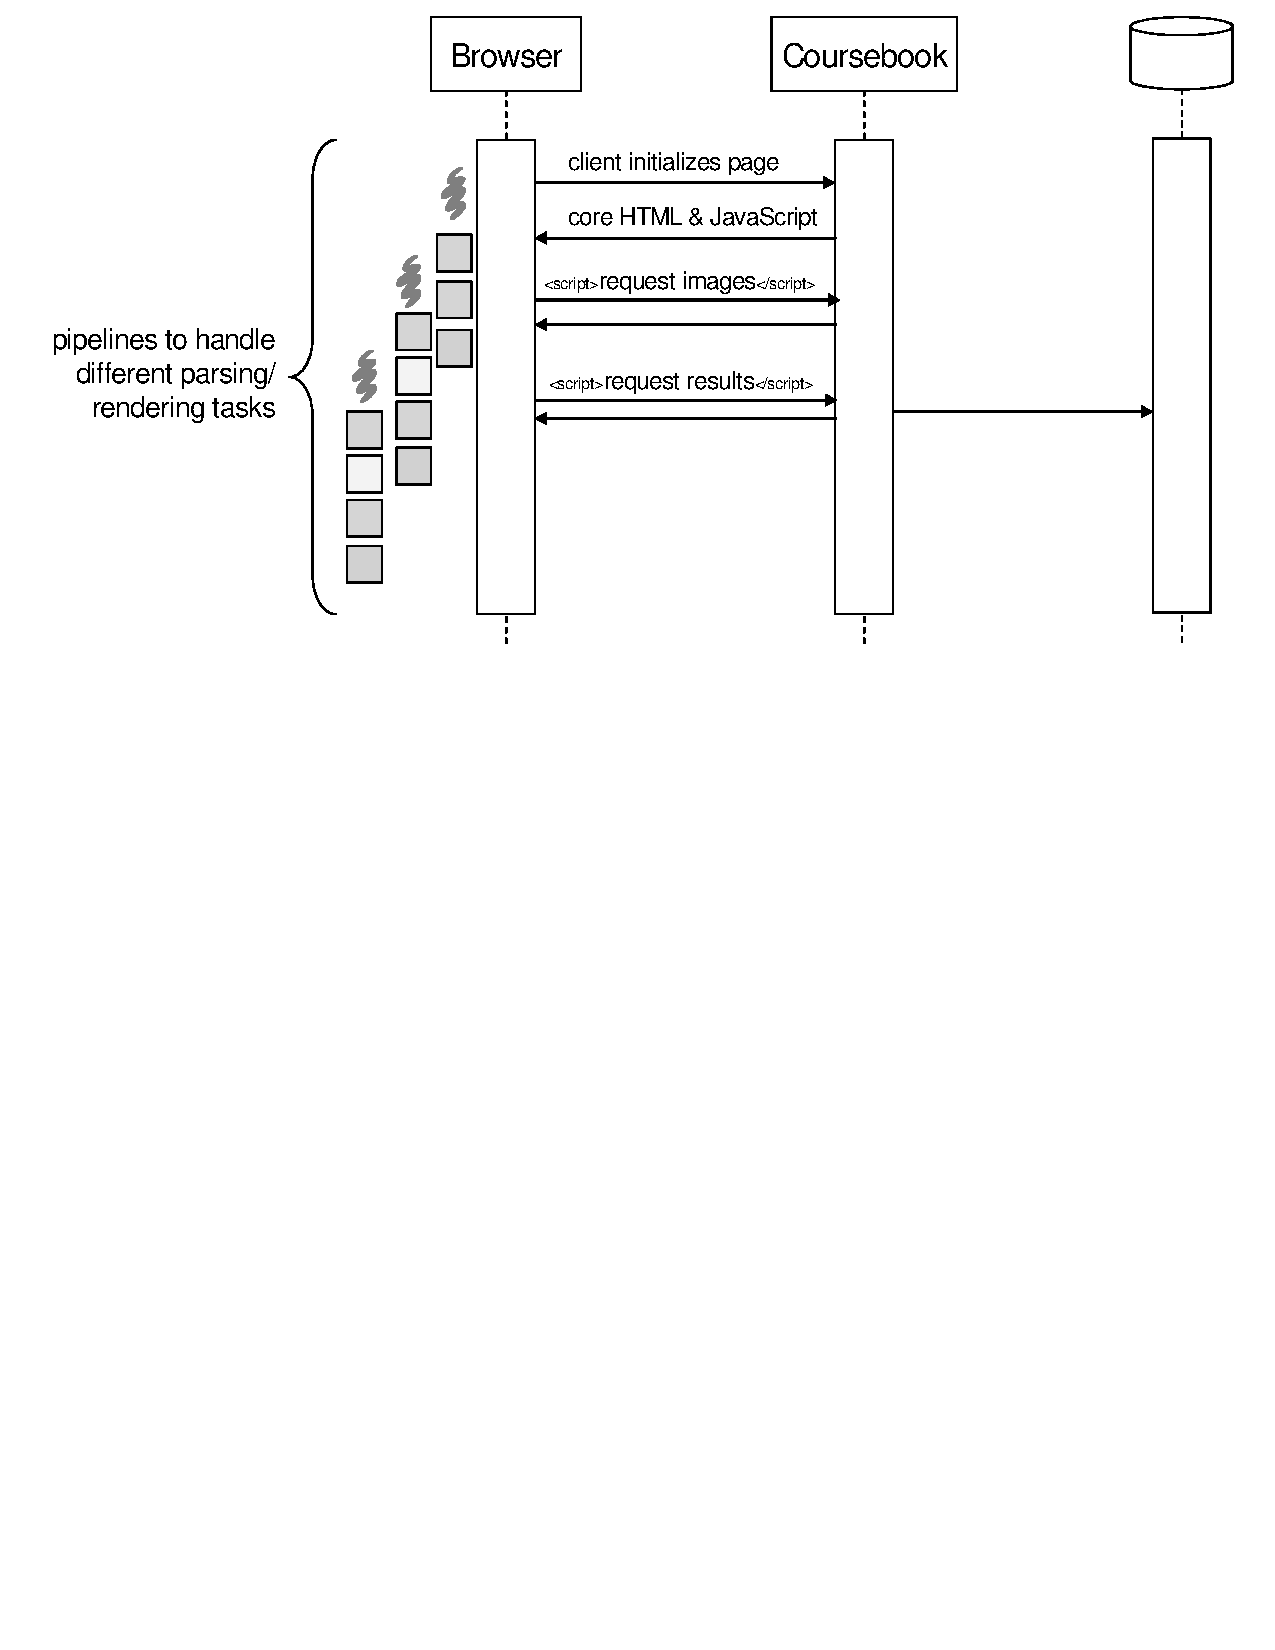
\includegraphics[width=\textwidth]{images/pipesequence}
  \caption{Sequence Diagram for Pipeline in Coursebook}
  \label{fig:pipesequence}
  \end{center}
\end{figure}

By introducing these sub-phases, we can perform multiple pipes of the entire
task at once. We will have three of these pipes running simultaneously to
decrease the perceived response time of our application. Figure
\ref{fig:pipesequence} shows the pipelining sequence for these phases. First, we
will start a pipe to download the Core UI and Javascript code. When this pipe
completes, the initial user interface will be rendered and the user will
\textit{feel} like their application is ready to use. While the first pipe for
the Core UI is executing, we will start another pipe for downloading and
rendering images. This is the second group of phases that we will execute in our
pipeline. The client web browser will dowload the Javascript code, and actively
request data for images then render the page. While this is happening, the
client invokes a third request for results to start the third set of tasks in
the pipe. Our server queries the database to search for appropriate courses. 
When they are ready, the final pipe downloads and renders the results.
